% Automatisch erzeugt von bom_pdf.py -- Änderungen hier gehen beim
% nächsten Lauf verloren. Inhalte in bom.csv und versionshistorie.txt pflegen.
\documentclass[11pt,a4paper]{scrartcl}
\usepackage[utf8]{inputenc}
\usepackage[T1]{fontenc}
\usepackage[german]{babel}
\usepackage{lmodern}
\usepackage{textcomp}
\usepackage{geometry}
\usepackage{longtable}
\usepackage{array}
\usepackage{graphicx}
\usepackage{booktabs}
\geometry{a4paper,left=25mm,right=25mm,top=30mm,bottom=25mm}
\setlength{\parindent}{0pt}
\pagestyle{plain}
\begin{document}
\begin{titlepage}
  \begin{center}
    {\large Wilhelm Büchner University of Applied Sciences} \\[0.3em]

    {\normalsize Projektseminar Master}
\vspace{5em}

    {\LARGE\bfseries Coasterbot} \\[0.5em]

    {\large Stückliste - BOM} \\[1em]

    {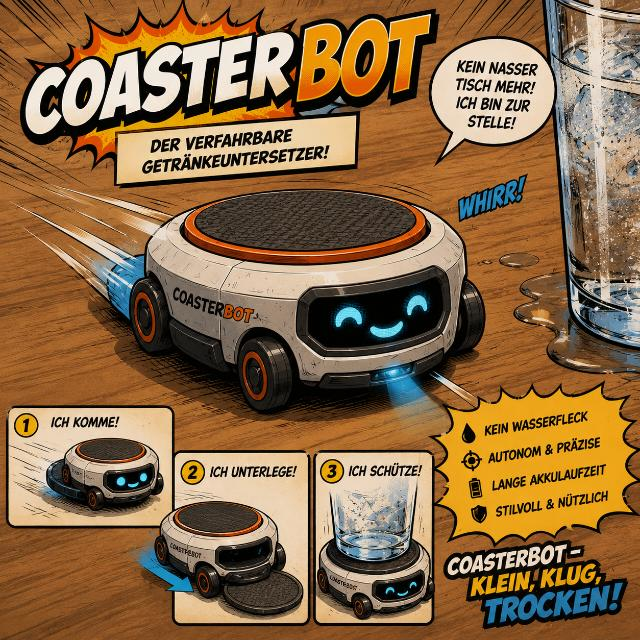
\includegraphics[width=0.38\textwidth]{coasterbot.png}} \\[1em]

\vspace{4em}

    {\normalsize
\begin{tabular}{ll}
Dennis Borutta, B. Eng & dennis.borutta@outlook.com\\
Stefan Etringer, B. Eng & mail@stefan.works\\
Gereon Such, M. Sc. & gereonsuch@gmail.com\\
\end{tabular}
    }
  \end{center}
\end{titlepage}

\section*{Versionshistorie}
\begin{tabular}{@{}p{1.6cm}p{2.4cm}p{3.0cm}>{\raggedright\arraybackslash}p{7.0cm}@{}}
\toprule
\textbf{Version} & \textbf{Datum} & \textbf{Bearbeiter} & \textbf{Änderung}\\
\midrule
1 & 24.08.2026 & Such & Erstfassung der Stückliste, Merge von Elekronik und Mechanik\\
2 & 25.08.2026 & Such & RGB LED und Taster eingefügt\\
\bottomrule
\end{tabular}
\clearpage

% Querformat: geometry kann die Papiergröße nachträglich nicht ändern,
% daher werden Seitenmaße und Satzspiegel hier direkt gesetzt.
\paperwidth=297.0mm
\paperheight=210.0mm
\pdfpagewidth=\paperwidth
\pdfpageheight=\paperheight
\setlength{\hoffset}{0pt}
\setlength{\voffset}{0pt}
\setlength{\headheight}{0pt}
\setlength{\headsep}{0pt}
\setlength{\oddsidemargin}{-10.40mm}
\setlength{\evensidemargin}{-10.40mm}
\setlength{\topmargin}{-10.40mm}
\setlength{\textwidth}{267.00mm}
\setlength{\textheight}{180.00mm}
% Satzspiegel-Änderungen mitten im Dokument wirken nur, wenn die davon
% abgeleiteten Maße mitgezogen werden.
\setlength{\columnwidth}{\textwidth}
\setlength{\linewidth}{\textwidth}
\setlength{\hsize}{\textwidth}
\setlength{\vsize}{\textheight}
\makeatletter
\global\@colht=\textheight
\global\@colroom=\textheight
\makeatother
\setlength{\tabcolsep}{2.12mm}
\renewcommand{\arraystretch}{1.2}
\footnotesize
\begin{longtable}{@{}>{\raggedleft\arraybackslash}p{16.74mm}>{\raggedleft\arraybackslash}p{15.76mm}>{\raggedright\arraybackslash}p{14.77mm}>{\raggedright\arraybackslash}p{44.31mm}>{\raggedright\arraybackslash}p{25.60mm}>{\raggedright\arraybackslash}p{76.81mm}>{\raggedleft\arraybackslash}p{21.66mm}>{\raggedleft\arraybackslash}p{21.66mm}@{}}
\toprule
\textbf{Position} & \textbf{Menge} & \textbf{Einheit} & \textbf{Benennung} & \textbf{Sachnummer} & \textbf{Bemerkung} & \textbf{Einzelpreis} & \textbf{Gesamtpreis}\\
\midrule
\endfirsthead
\toprule
\textbf{Position} & \textbf{Menge} & \textbf{Einheit} & \textbf{Benennung} & \textbf{Sachnummer} & \textbf{Bemerkung} & \textbf{Einzelpreis} & \textbf{Gesamtpreis}\\
\midrule
\endhead
\bottomrule
\endfoot
\bottomrule
\endlastfoot
1 & 1 & Stk. & Gehäuse und Coaster &  & 420g PLA im 3D Druck, Einzelpreis ist kg Preis & 9.74€ & 4.09€\\
2 & 24 & Stk. & Gewindeschraube & M2.3x8 & Verbindung der Teile & 0.02€ & 0.48€\\
3 & 2 & Stk. & Gewindeschraube & M2.3x10 & Drehpunkt des Schiebers & 0.02€ & 0.04€\\
4 & 40 & Stk. & Neodymium Magnete &  & Wzone 5x2mm Small Magnet; Für Coaster und Heber & 0.06€ & 2.40€\\
5 & 1 & Stk. & Microcontroller & U2 & Raspberry Pi Pico2 Microcontroller Dev-Board & 14.00€ & 14.00€\\
6 & 1 & Stk. & DC/DC Step Up converter & U1 & VISSQH; Akku 3.7V nach 5V Vcc & 0.60€ & 0.60€\\
7 & 2 & Stk. & DC Motor Treiber & U3, U4 & TB6612FNG Entwicklungsboard & 4.20€ & 8.40€\\
8 & 4 & Stk. & TT Motor & U5, U6, U7, U8 & GUUZI DC Motor 3-6V mit 1:48 Getriebe und Rad & 3.25€ & 12.99€\\
9 & 2 & Stk. & Tischkanten-Sensor & U9, U10 & EBKSQS IR Infrared Obstacle Sensor zur Tischkantenerkennung vor Frontantrieb & 1.50€ & 3.00€\\
10 & 1 & Stk. & Hindernis-Sensor & U11 & HC-SR04, Ultraschall Sensor zur Montage in Fahrtrichtung & 1.50€ & 1.50€\\
11 & 1 & Stk. & Inertialsensor & U12 & ICQUANZX GY-521 MPU6050; Navigationssensor & 5.59€ & 5.59€\\
12 & 2 & Stk. & Auswurf/Aufnahme Servo & U13, U14 & MT90 Servo & 2.20€ & 4.40€\\
13 & 1 & Stk. & Li-Ion Akku & BT1 & 18650 3.7V 1200mAh Akku inkl. Charger & 3.00€ & 3.00€\\
14 & 1 & Stk. & VM-Elko & C1 & 470uF Elektrolyt Kondensator & 0.30€ & 0.30€\\
15 & 1 & Stk. & VCC-Elko & C2 & 100uF Elektrolyt Kondensator & 0.10€ & 0.10€\\
16 & 4 & Stk. & Motor-Entstör Kondensator & C3, C4, C5, C6 & 100nF Keramik Kondensator zur Verhinderung von Induktionen beim Ändern der Antriebsrichtung & 0.04€ & 0.16€\\
17 & 1 & Stk. & Entprell Kondensator & C7 & 100nF Keramik Kondensator zum Entprellen des Nutzer-Tasters und Verhindern Einstreuung der Motoren & 0.054€ & 0.04€\\
18 & 1 & Stk. & Taster & SW2 & Gehäusemontage Taster & 0.50€ & 0.50€\\
19 & 1 & Stk. & Widerstand & R1 & Pullup Widerstand & 0.01€ & 0.01€\\
20 & 1 & Stk. & RGB LED & U15 & KY-016 RGB LED zur Status Anzeige, Modul zur einfacheren Montage gewählt & 0.78€ & 0.78€\\
21 & 1 & Stk. & Hauptschalter & SW1 & Gehäusemontage Schalter & 0.15€ & 0.15€\\
22 & 1 & Stk. & Hauptplatine &  & Lochrasterplatine zur Kombination von Microcontroller, Leistungselektronik und Steckverbindern & 0.89€ & 0.89€\\
23 & 9 & Stk. & Steckverbinder &  & Leitungen von Hauptplatine zu Sensorik & 0.05€ & 0.45€\\
24 & 1 & Stk. & Pfostenleiste &  & 1x40 Pol 2.54mm gerade, Verbindung von Modulplatinen mit Hauptplatine & 0.60€ & 0.60€\\
\midrule
\multicolumn{7}{@{}r}{\textbf{Gesamtbetrag je Prototyp}} & \textbf{64.47€}\\
\end{longtable}
\end{document}
